\documentclass{article}

% preambulo:
\usepackage[utf8]{inputenc}
% caracteres utf8 (tildes, enie) sin tener que usar comandos

\usepackage[spanish, es-tabla, es-nodecimaldot]{babel} 
% texto automatico en espaniol
% "tabla" en vez de "cuadro"
% no reemplaza puntos decimales por comas

%% NO AGREGAR PAQUETES ANTES DE ESTO, ES IMPORTANTE QUE BABEL ESTE PRIMERO

%%%%%%%%%%%%%%%%%%%%%%%%%%%%%%%%%
%% PAQUETES EXTRA %%%%%%%%%%%%%%%
%%%%%%%%%%%%%%%%%%%%%%%%%%%%%%%%%

\usepackage{subfiles}

\usepackage{amsmath} % PAQUETES DE MATEMATICA
\usepackage{amsfonts}
\usepackage{amssymb}


\usepackage{steinmetz} % comando \phase{}
\usepackage{units} % permite usar nicefrac
\usepackage{graphicx} % importar imagenes
\usepackage{float} % posicion H para floats
\usepackage[colorinlistoftodos]{todonotes}


\usepackage[a4paper, total={6in, 8in}]{geometry} 
% margenes correctos en subarchivos

\setlength{\parindent}{10pt}			%cuanta sangria al principio de un parrafo
\usepackage{indentfirst}				%pone sangria al primer parrafo de una seccion

\usepackage{listings}

%%%%%%%%%%%%%%%%%%%%%%%%%%%%%%%%%%%%%%%%%%%%%%%%%%%%%%%%%%%
%% NO AGREGAR PAQUETES DESPUES DE ESTO, ES IMPORTANTE QUE HYPERREF ESTE ULTIMO
\usepackage[hidelinks]{hyperref} % hipervinculos sin cajitas rojas




\begin{document}

\newgeometry{} % margenes default para la caratula
% caratula:
\begin{titlepage}
\newcommand{\HRule}{\rule{\linewidth}{0.5mm}}
\center
\mbox{\textsc{\LARGE \bfseries {Instituto Tecnol\'ogico de Buenos Aires}}}\\[1.5cm]
\textsc{\Large 22.99 Laboratorio de Microprocesadores}\\[0.5cm]


\HRule \\[0.6cm]
{ \Huge \bfseries Guía de Ejercicios N$^{\circ}$2: Introducción a Kinetis}\\[0.4cm] % Title of your document
\HRule \\[1.5cm]


{\large

\emph{Grupo 2}\\
\vspace{3px}

\begin{tabular}{lr} 	
\textsc{M\'aspero}, Martina  & 57120 \\
\textsc{Mestanza}, Joaqu\'in Mat\'ias  & 58288 \\
\textsc{Nowik}, Ariel Santiago  & 58309 \\
\textsc{Regueira}, Marcelo Daniel  & 58300 \\
\end{tabular}

\vspace{20px}

\emph{Profesores}\\
\vspace{3px}
\textsc{Jacoby}, Daniel Andr\'es\\ 	
\textsc{Magliola}, Nicol\'as\\ 	

\vspace{100px}

\begin{tabular}{ll}

Presentado: & 22/08/2019\\

\end{tabular}

}

\vfill

\end{titlepage}

% cambio los margenes para el resto del documento
\newgeometry{left=2.5cm, top=2.5cm, right=2cm, bottom=2cm}

% indice:
\tableofcontents
\newpage

\section*{Ejercicio 1}

\begin{itemize}
\item ¿En cuál número de pin del MCU se encuentra el puerto PTA12?
\end{itemize}
En el datasheet del MCU, la sección 5.3 ``K64 Pinouts'' figura 37, se indica que el puerto PTA12 es el pin 64.

\begin{itemize}
\item ¿Cuáles pines pueden funcionar como entradas analógicas?
\end{itemize}
En el datasheet del MCU, la sección 5.2 ``Unused analog interfaces'' tabla 57, indica el nombre del módulo y los pines asociados:

\begin{figure}[ht]
	\centering
	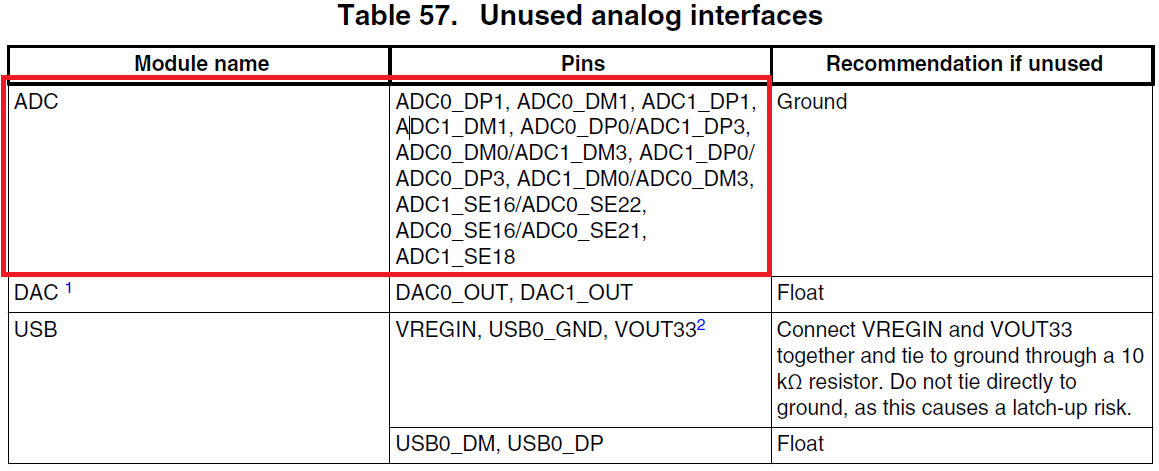
\includegraphics[width=0.8 \textwidth]
	{../Imagenes/TablaADC.png}
	\caption{Pines de entrada analógica}
	\label{fig:ej1}
\end{figure}

\begin{itemize}
\item ¿Cuántos pines del puerto PTE se encuentran efectivamente disponibles en este modelo de MCU?
\end{itemize}
En la guía de usuario del kit Freedom, sección 16 ``Input/output connectors'' se muestran los pintes accesibles en la placa de evaluación. Los pines disponibles de uso externo del puerto PTE son el PTE24, PTE25 y el PTE26.

\begin{itemize}
\item ¿Cuál es el rango de valores de tensión para detectar un 0 y un 1 lógico en un pin I/O? ¿Se puede enviar 5V a un pin?
\end{itemize}
En el datasheet del MCU, la sección 2.2.1 ``Voltage and current operating requirements'' tabla 1 se indican los márgenes de ruido correspondientes:

\begin{figure}[ht]
	\centering
	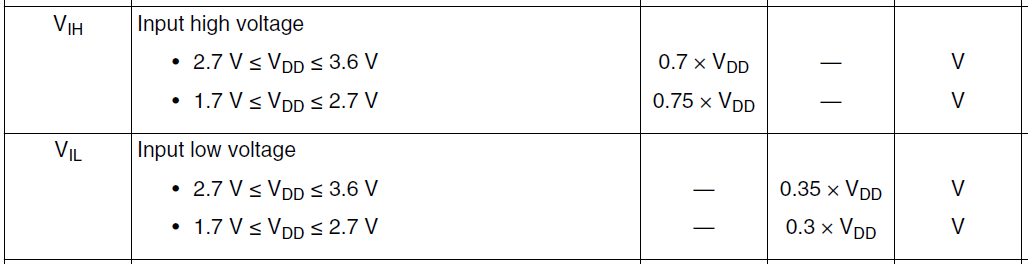
\includegraphics[width=0.8 \textwidth]
	{../Imagenes/TablaMargenes.png}
	\caption{Márgenes de ruido}
	\label{fig:ej1}
\end{figure}

Por otro lado, en el datasheet del MCU, la sección 1.4 ``Voltage and current operating ratings'', en el cuadro se indica que la máxima tensión de entrada a un pin I/O es de 5.5V.

\begin{itemize}
\item ¿Cuál es la máxima corriente que entrega un pin I/O?
\end{itemize}
En el datasheet del MCU, la sección 1.4 ``Voltage and current operating ratings'', en el cuadro se indica que la máxima corriente por un pin I/O es de 25mA.

\newpage

\section*{Ejercicio 2}

Con el nivel de optimización original (None - O0), el código funciona normalmente. Con la opción Disassembly se puede obtener el fragmento de código de la función App\_run:

\begin{lstlisting}
          App_Run:
00000410:   push    {r7, lr}
00000412:   add     r7, sp, #0
00000414:   ldr     r0, [pc, #12]   ; (0x424 <App_Run+20>)
00000416:   bl      0x6b0 <delayLoop>
0000041a:   movs    r0, #154        ; 0x9a
0000041c:   bl      0x658 <gpioToggle>
00000420:   nop     
00000422:   pop     {r7, pc}
00000424:   rev     r0, r0
00000426:   lsls    r3, r3, #3
\end{lstlisting}

En el cual se observa que el compilador procesa la función delayloop correctamente. En cambio, utilizando la opción Optimize Most - O3, el compilador elimina esa función dado que bloquea el programa (y puede realizarse lo mismo con un timer). En consecuencia queda solamente el toogle corriendo todo el tiempo sin delay, por lo que no se llega a ver el blink.

\begin{lstlisting}
          App_Run:
00000418:   movs    r0, #154        ; 0x9a
0000041a:   b.w     0x614 <gpioToggle>
0000041e:   nop     
\end{lstlisting}

\newpage

\section*{Ejercicio 3}

Para utilizar el LED verde del RGB, se modificó el define correspondiente a dicho puerto, en board.h:

\begin{lstlisting}
#define PIN_LED_GREEN   PORTNUM2PIN(PE,26) // PTE26
\end{lstlisting}

En base a esto, se modificó también el código en App.c:

\begin{lstlisting}
/* Funcion que se llama 1 vez, al comienzo del programa */
void App_Init (void)
{
    gpioMode(PIN_LED_GREEN, OUTPUT);
}

/* Funcion que se llama constantemente en un ciclo infinito */
void App_Run (void)
{
    delayLoop(4*3600000UL);
    gpioToggle(PIN_LED_GREEN);
}
\end{lstlisting}

El valor en delayloop se modificó por prueba y error, dado que es un while que incrementa una variable, y para conocer el tiempo que demora se midió el del código de blink con el osciloscopio, que era delayloop(4000000UL). La forma más adecuada de implementar un retardo en el cambio de estado de un pin sería utilizando un timer.

\end{document}
